\section{Design of the System}
\label{sec:design}

Small description :
\begin{mylist}
\item \textbf{Find program point for patching.} We have used static taint
analysis to detect if a particular statement is on the path from tainted source
to sink. In such case we have excluded it from repairing. Also we have performed
analysis on call graph to detect if there is already handled exception placed by
the developer or not. In such cases also we have considered such statement tot
to patch.

\item \textbf{Static constraint analysis.} We have collected and evaluated
constraint for such conditional expression for which we can evaluate them
statically to make sure the patched object have the correct characteristics.

\item \textbf{Patching.} We have find such statements which can potentially throw
\code{RuntimeException} and we put them in try-catch block and place appropriate
patch inside the catch block based on the appropriate exception type.

\item \textbf{Dynamic constraints.} Apart form static constraint evaluation,
there may be some constraint in the program which depends on the user input
value which can not be determined statically. For such cases we have also
instrumented dynamic constraint collection statements in the program which will
collect and evaluate objects at runtime. These newly instrumented statements
will also collect the static constraint information to ensure correctness in
constraint evaluation.

\end{mylist}
%later convert this pdf
\begin{figure}[t]
\centering
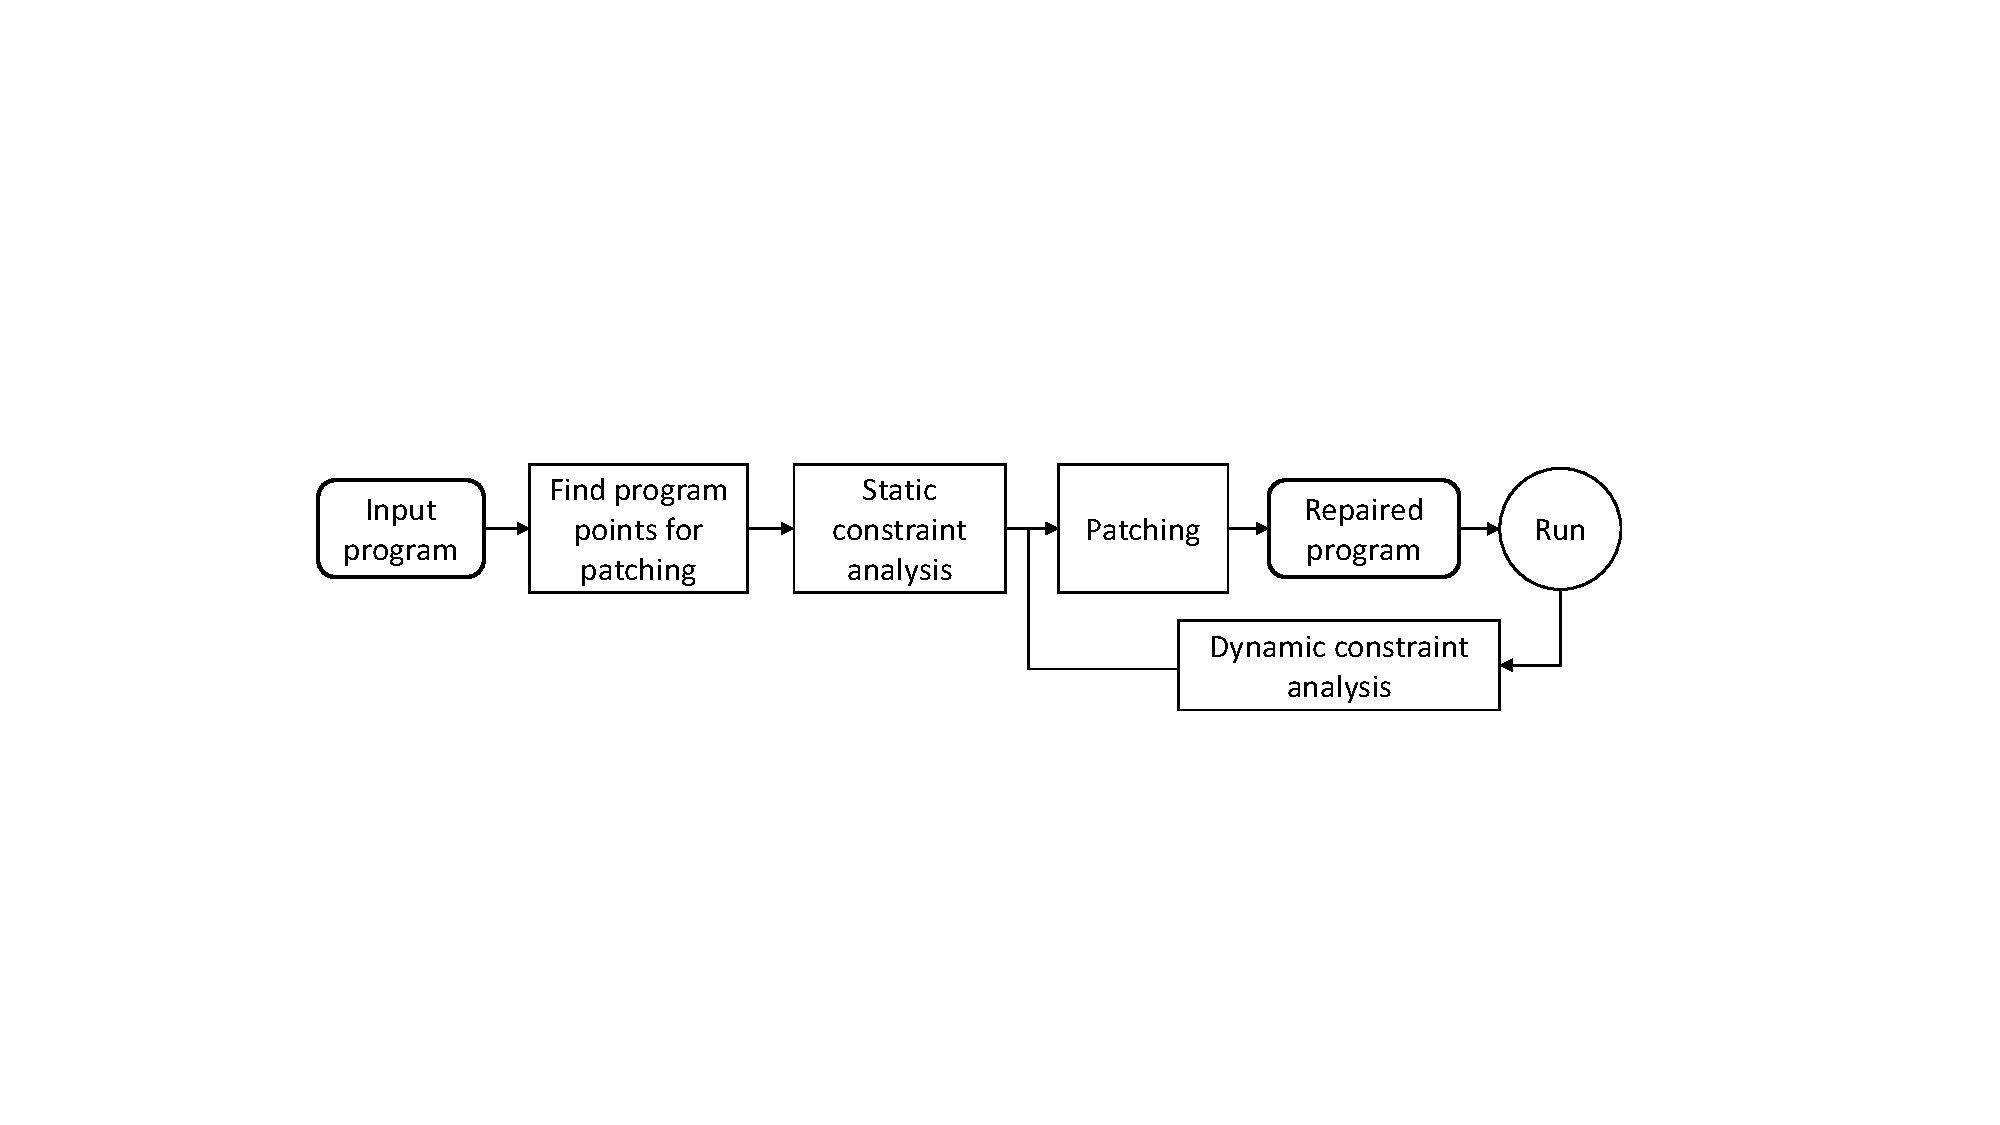
\includegraphics[scale=.38]{images/NewDesignDiagram.pdf}
\caption{Overall Design}
\label{fig:overallDesign}
\end{figure}


% \begin{figure}[!htb]
% \centering
% 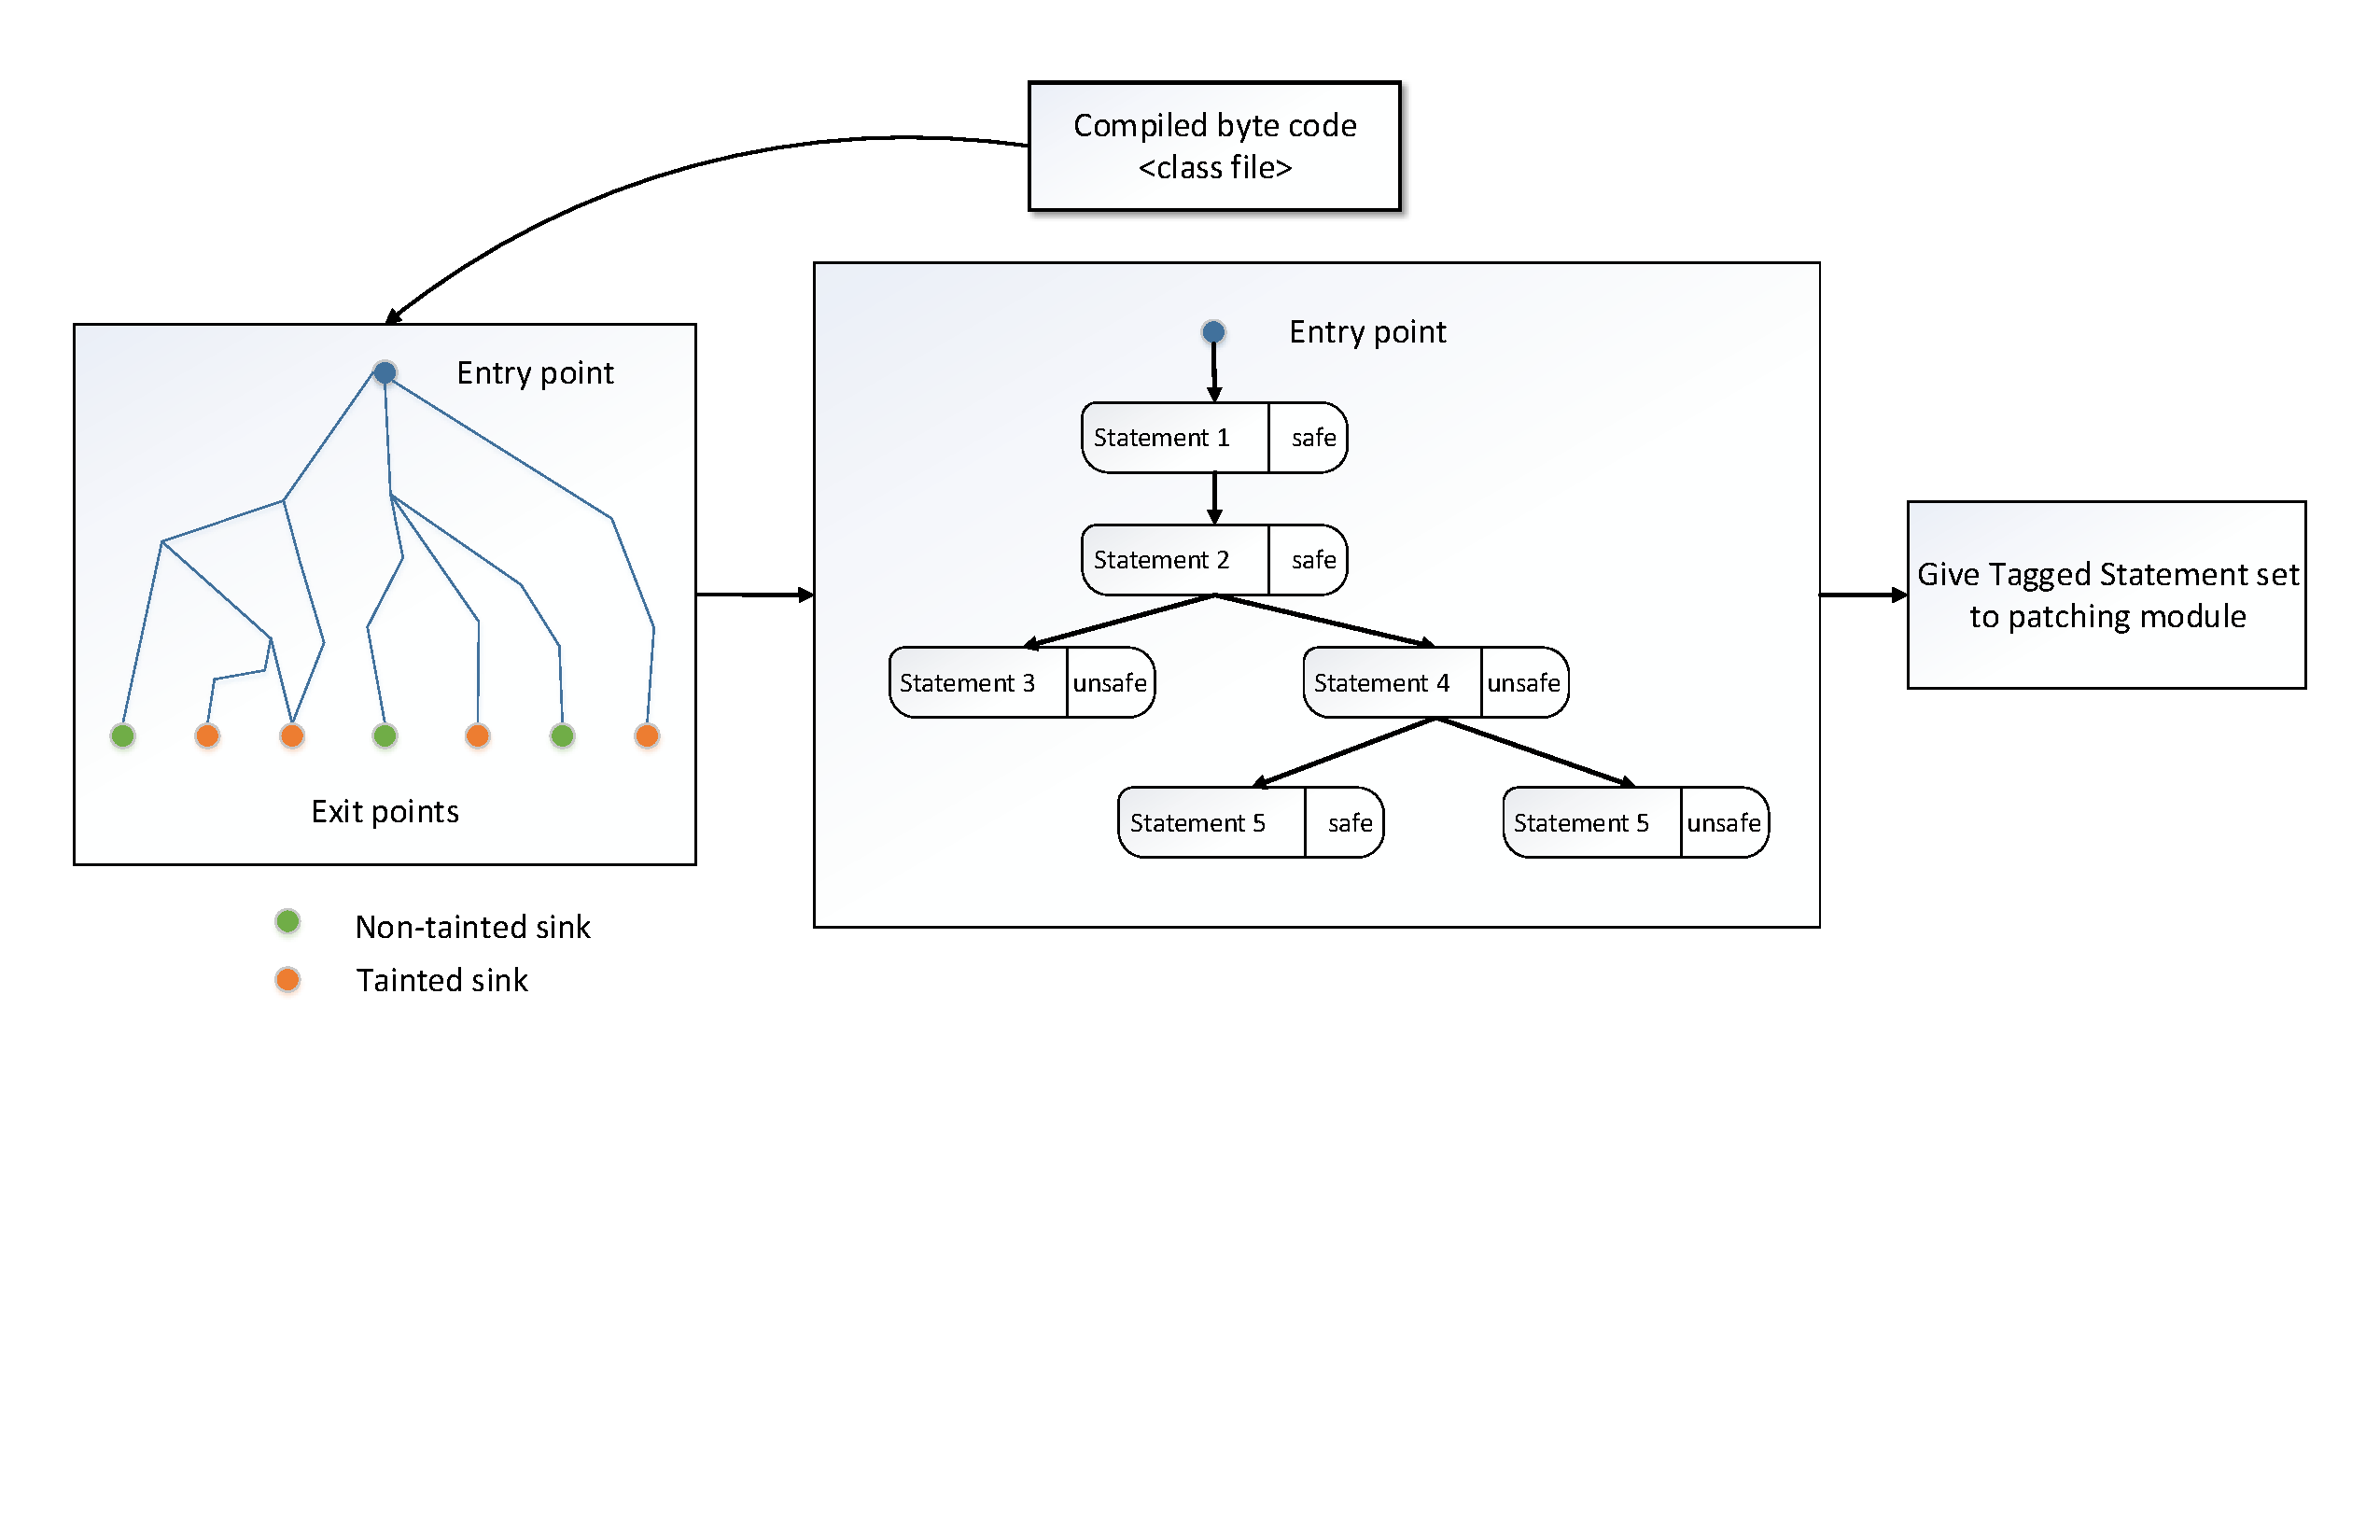
\includegraphics[width=3.5in]{images/TaintModule.pdf}
% \caption{Overall Design}
% \label{fig:TaintModule}
% \end{figure}
% 
% \begin{figure*
%   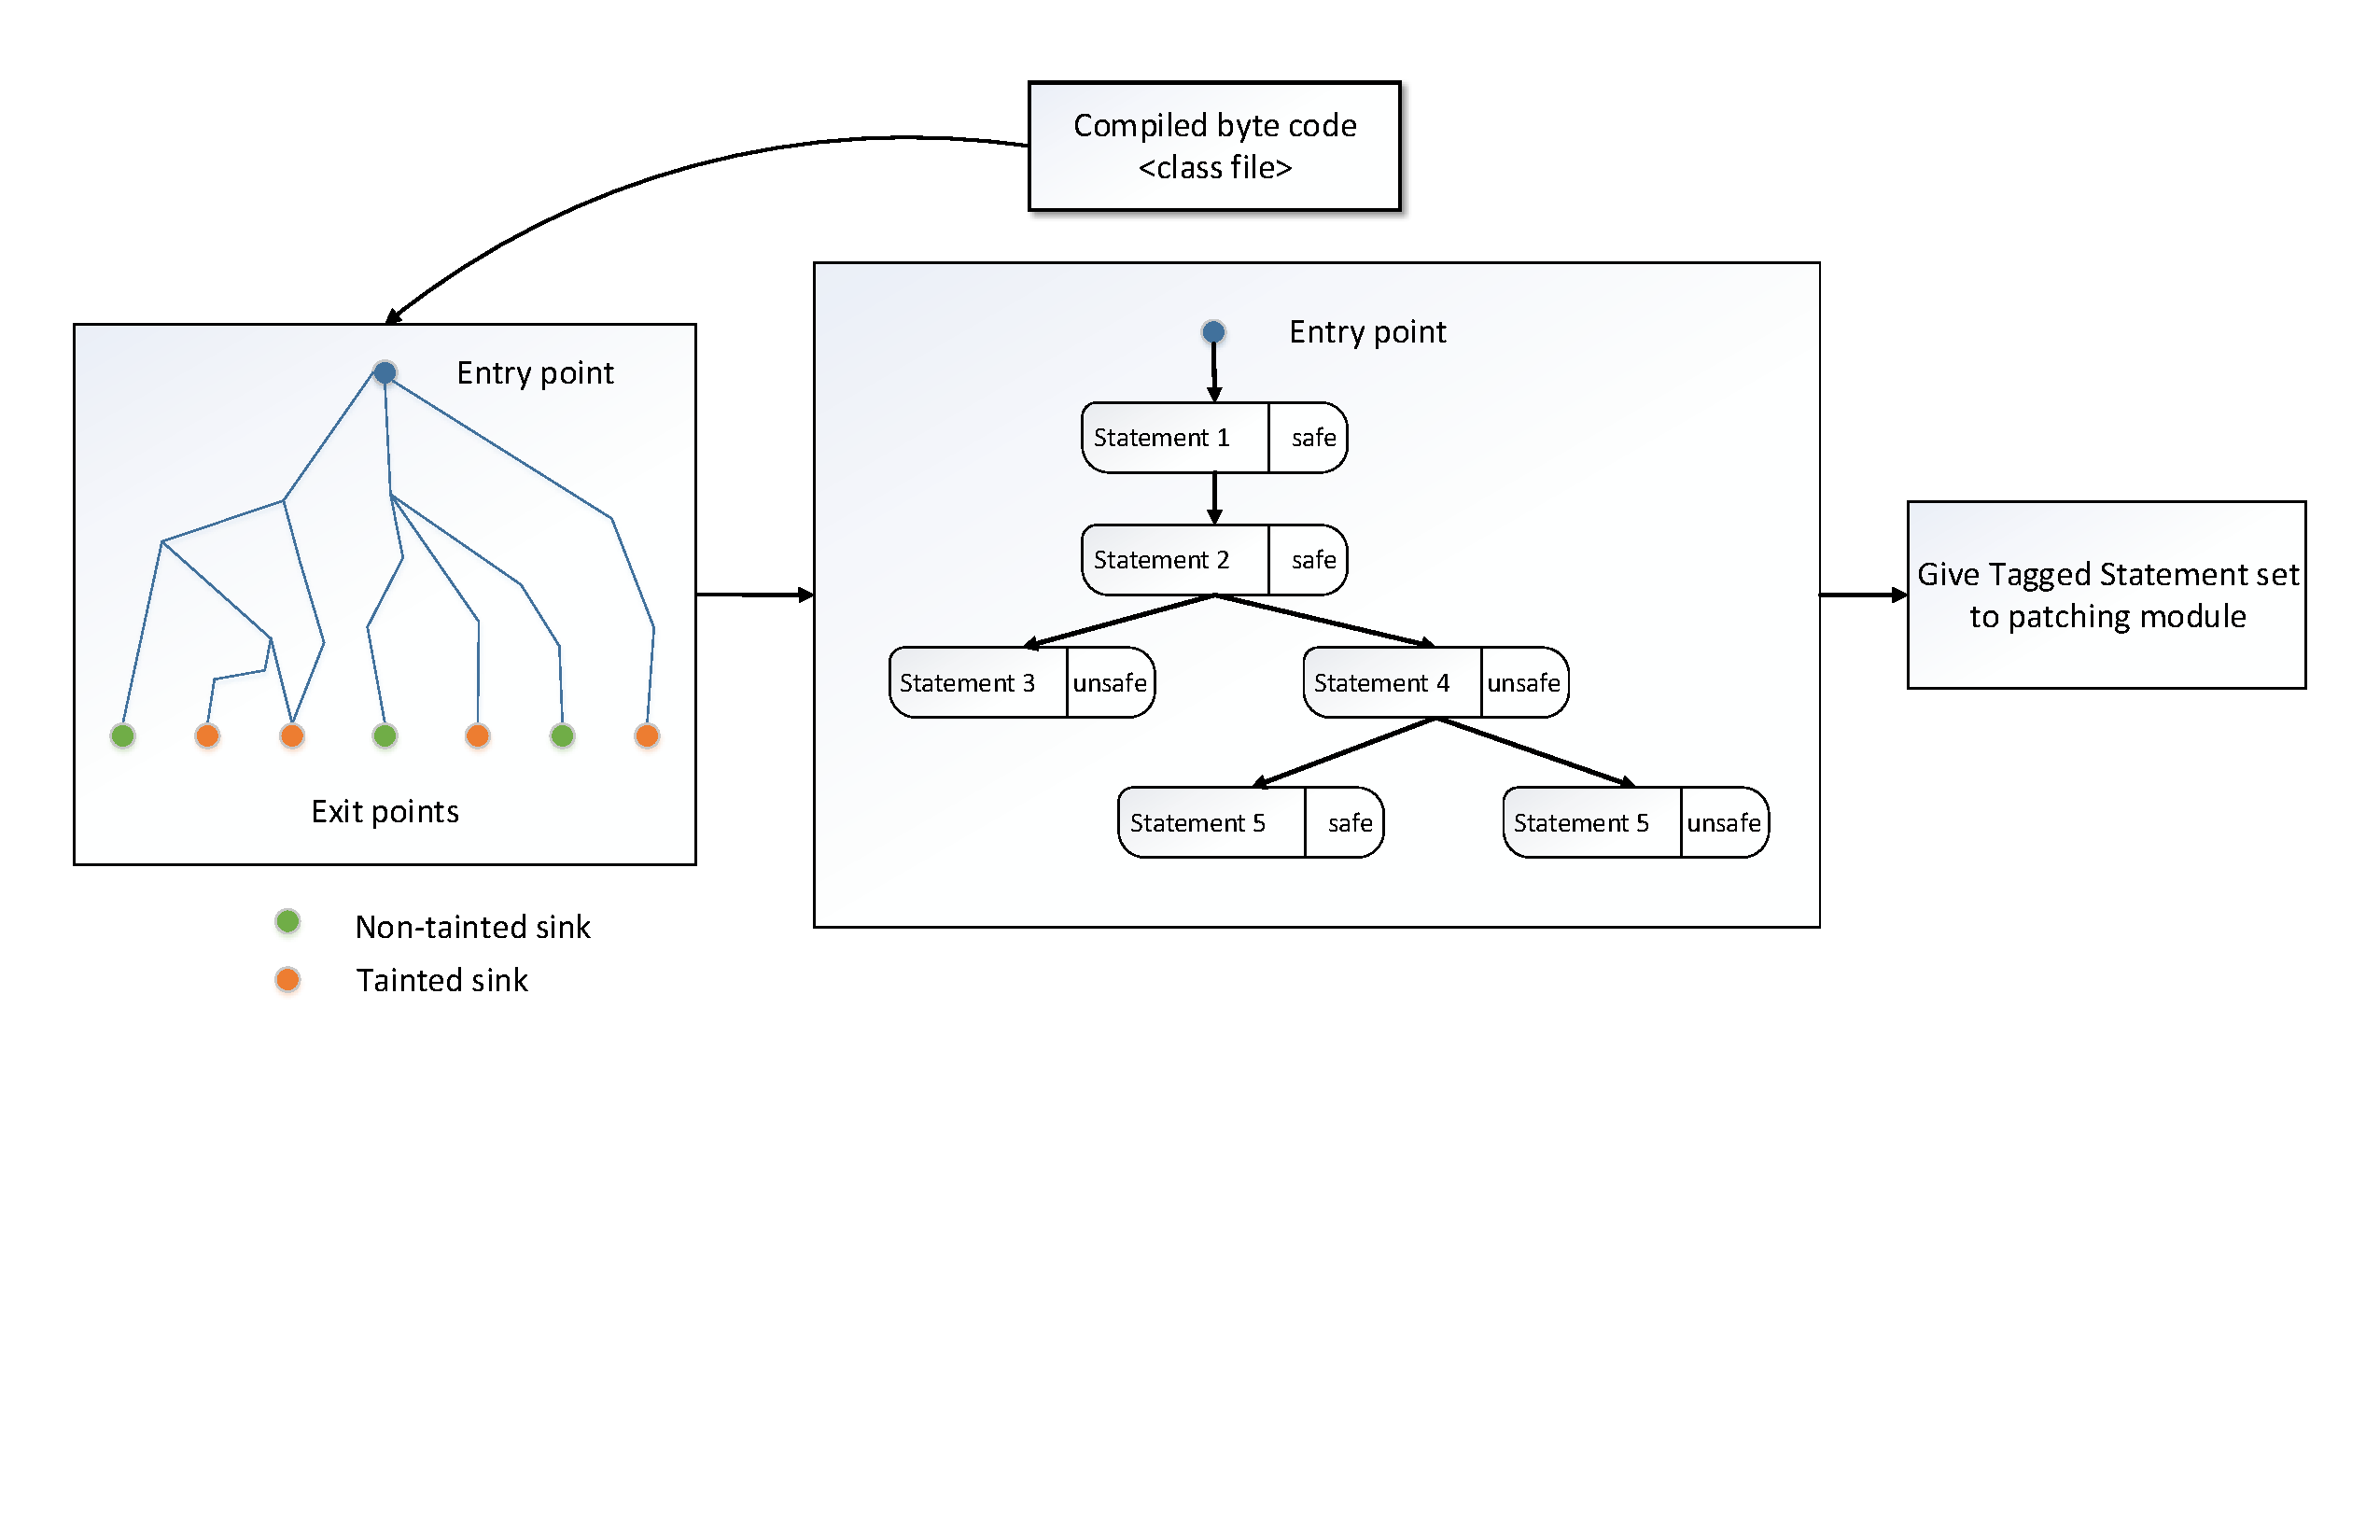
\includegraphics[width=\textwidth,height=5cm]{images/TaintModule.pdf}
%   \caption{Design of the Taint Module}
% \end{figure*}

%later covert this to pdf
\begin{figure*}[t]
\centering
  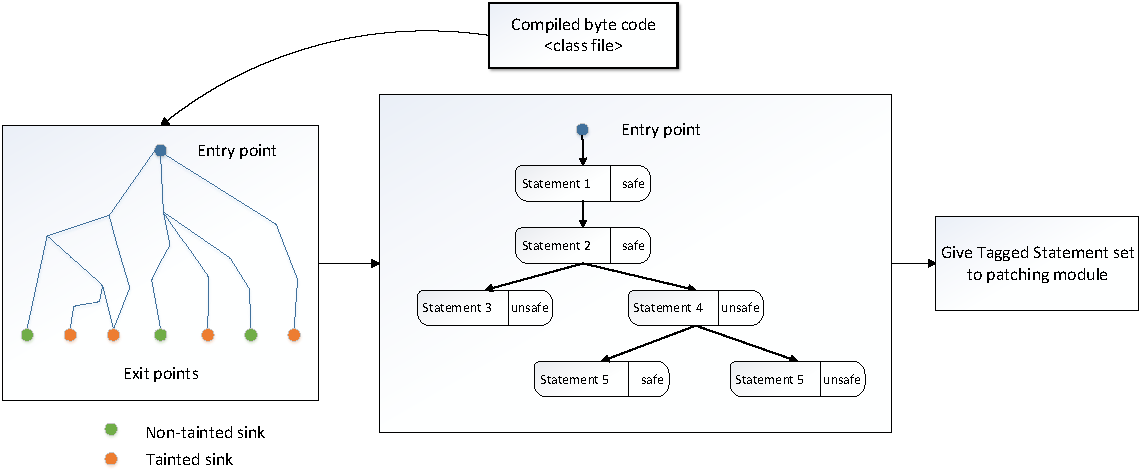
\includegraphics[scale= .4]{images/TaintModule.png}
  \caption{Design of the Taint Module}
  \label{fig:TaintModule}
\end{figure*}


The overall design of the repairing framework is illustrated in
Figure~\ref{fig:overallDesign}. The framework consists of four basic modules.


\subsection{Taint analysis Module}
\label{subsec:TaintModule}

The main purpose of the taint analysis module is to classify which of the
statements are safe to patch or not. Based on the analysis result in this
module, the tagged statement will be passed to the repairing module.


We have specify the list of source, sink and derivation methods in a
configuration file before the analysis. The source methods includes methods
which
take input from user from console or web application forms like text box. The
sink methods are sensitive data storage which are unsafe to manipulate such as
database, console print or methods to send a text file to printer etc. The
overview of the taint analysis module is illustrated in the
Figure~\ref{fig:TaintModule}.  The input for the module is the compiled byte
code intended to be repaired. Here we have generated a control flow graph (CFG)
from to get all the possible program paths. The module will return all the
program statements which are on any of the program paths from source to sink.


\subsubsection{Tainting Rules}
\label{subsubsec:TaintingRule}
%\textcolor{red}{\textbf{Needs Revision}}\newline

\begin{table}[t]
\centering
\small
\begin{tabular}{l|l}
\multicolumn{1}{c|}{\textbf{\java\ Class}} & \multicolumn{1}{c}{\textbf{Source
Method}}\\
% \scalebox{0.86}
% {
\hline
\code{java.io.InputStream} & \code{read()}\\
\code{java.io.BufferedReader} & \code{readLine()}\\
\code{java.net.URL} & \code{openConnection()}\\
\code{org.apache.http.HttpResponse} & \code{getEntity()}\\
\code{org.apache.http.util.EntityUtils} & \code{toString()}\\
\code{org.apache.http.util.EntityUtils} & \code{toByteArray()}\\
\code{org.apache.http.util.EntityUtils} & \code{getContentCharSet()}\\
\code{javax.servlet.http.HttpServletRequest} & \code{getParameter()}\\
\code{javax.servlet.ServletRequest} & \code{getParameter()}\\
\code{java.Util.Scanner} & \code{next()}\\
\end{tabular}
\caption{Common \java\ library taint source functions}
\label{tab:TaintSources}
% }
\end{table}



\begin{table}[t]
\centering
\small
\begin{tabular}{l|l}
\multicolumn{1}{c|}{\textbf{\java\ Class}} & \multicolumn{1}{c}{\textbf{Sink
Method}}\\
% \scalebox{0.86}
% {
\hline
\code{java.io.PrintStream} & \code{printf()}\\
\code{java.io.OutputStream} & \code{write()}\\
\code{java.io.FileOutputStream} & \code{write()}\\
\code{java.io.Writer} & \code{write()}\\
\code{java.net.Socket} & \code{connect()}\\
%org.apache.http.impl.client.DefaultHttpClient & execute\\ \hline
\end{tabular}
% }
\caption{Common \java\ library taint sink functions}
\label{tab:TaintSinks}
\end{table}

~\newline

For any generic taint analysis, the tainting rules including a list of source 
and sink is to be defined. For our analysis we applied these policies, 

\begin{mylist}
  \item We defined list of source and sink taint methods listed in
  Table~\ref{tab:TaintSources} and \ref{tab:TaintSinks}. We are only tainting
  the variables which are coming from the listed taint source methods.
  
  \item We have also listed all taint propagation methods. The assignment ($=$)
  is the basic taint propagator. But there are other methods like \code{append}
  in \code{java.lang.StringBuffer} and \code{java.lang.StringBuilder} which are
  taint propagator.

  \item All the variable which are referred to tainted variables/ objects or
  output of taint propagator over tainted variable/objects are also considered
  as tainted.

  \item For all the program patch we see if such tainted variables are reaching
  the tainted sink or not. If they are reaching to some tainted sink then all
  the statements along that particular program path to which the tainted
  variables are assigned are marked as unsafe otherwise safe.
\end{mylist}


\subsection{Repairing Module}
\label{subsec:RepairingModule}

%later covert this to pdf
\begin{figure}[t]
\centering
  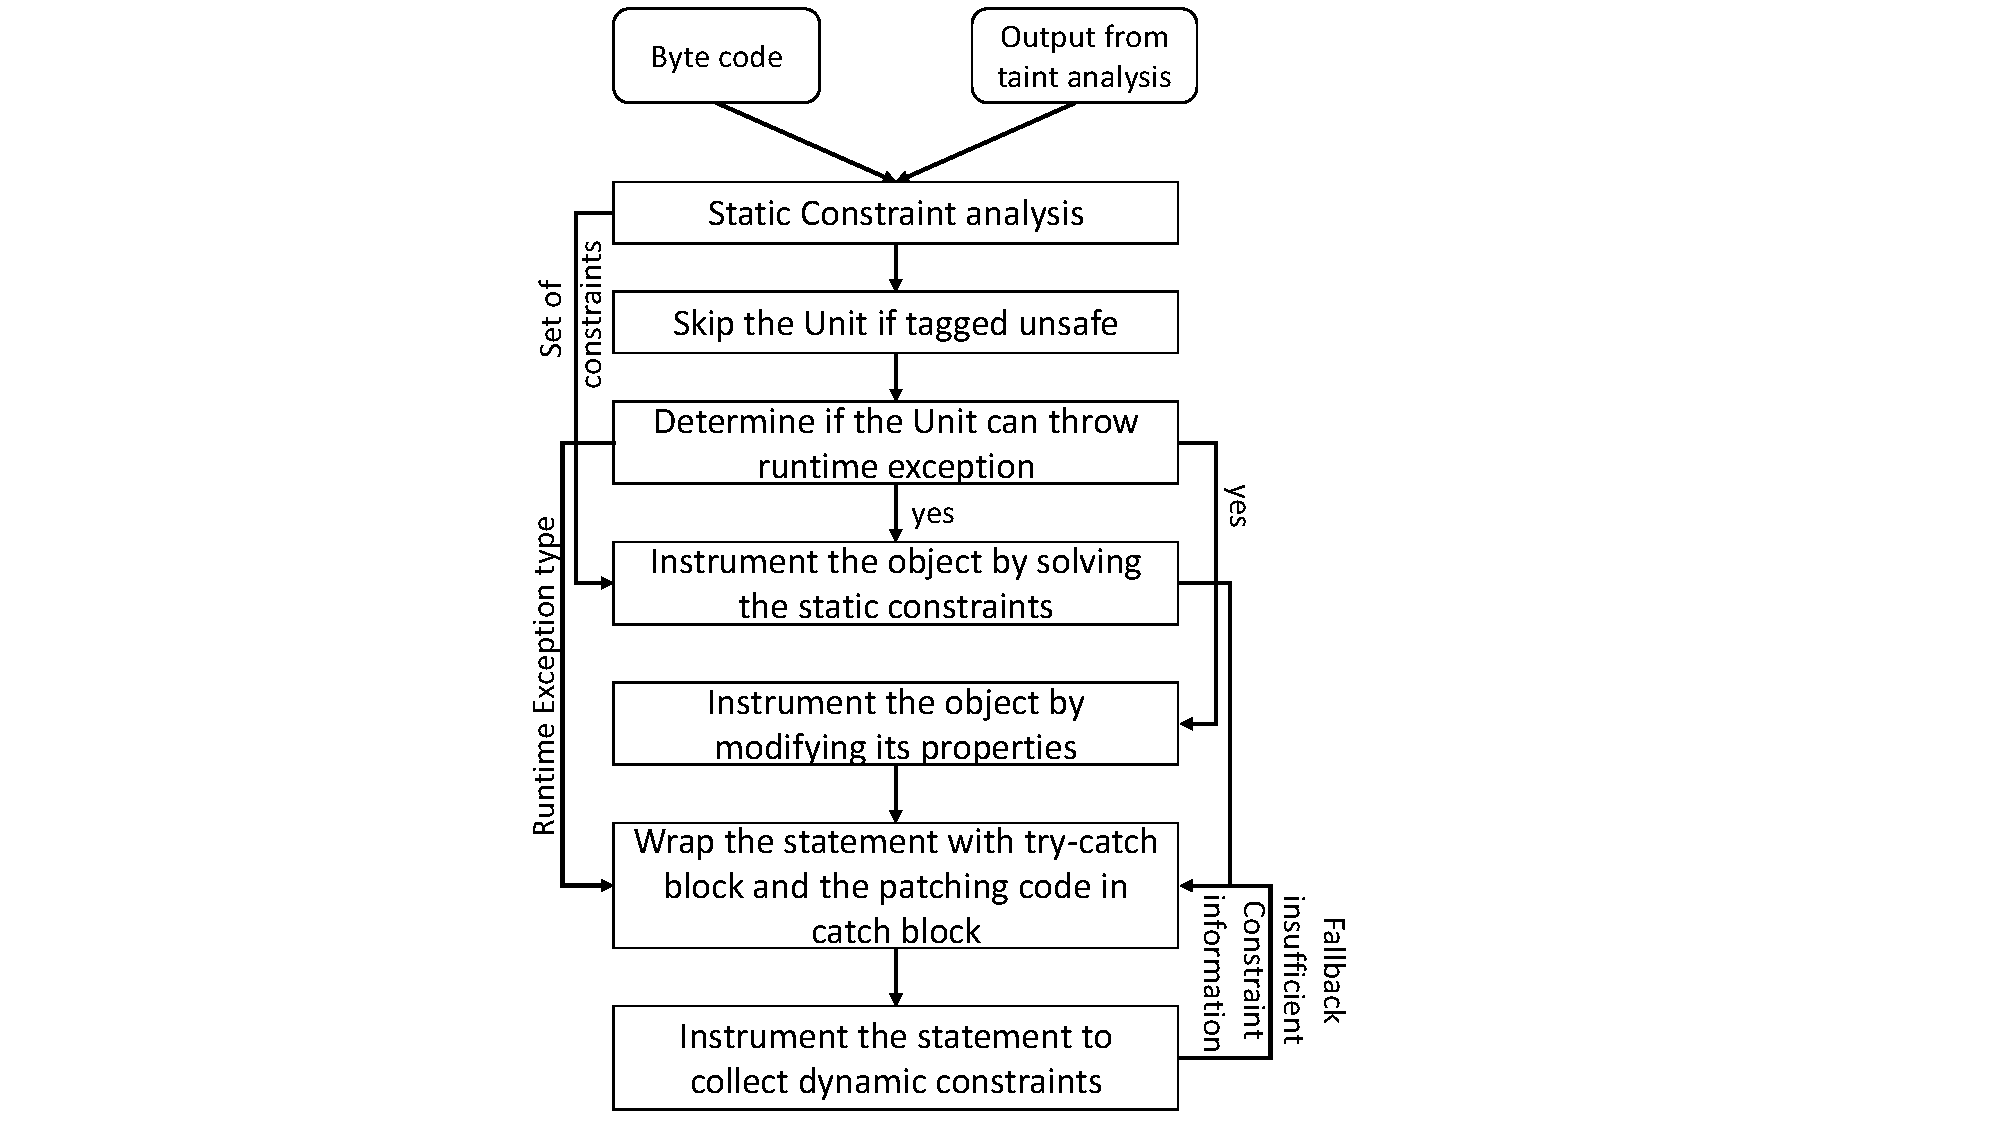
\includegraphics[scale= .4]{images/PatchModule.pdf}
  \caption{Design of the Patching Module}
  \label{fig:PatchModule}
\end{figure}

The repairing module is consisted of three phases. All these three phases
requires three sequential passes over the input bytecodes to produce the final
patched result.

\ignore{

\subsubsection{Example Scenario}
\label{subsec:exampleScenario}
~\newline
We have performed dataflow analysis by extending Soot main class. The objectives
of the dataflow analysis are the following:

\begin{itemize}
  \item For a target statement analyze used and defined variables.
  
  \item Extracts other statements which are both above and bellow the target
  statement in the control flow graph on which the used and defined variables
  are dependent on.
  
\end{itemize}

In the code snippet~\ref{snippet:dataflow}, we gave an example code based on
\java\ \code{String} API to demonstrate the analysis.


\lstset{language=Java, caption=Dataflow analysis, label = snippet:dataflow}
\begin{figure}[t]
\begin{lstlisting}
void bar() {
    foo("fname:lname");
}

String foo(String s) {
    int a = s.indexof(":");
    int b = s.indexOf("&");
    int c = s.indexOf("#");
    int d = 0;
    if(c>0)
	d = 1;
    return s.substring(a,b);
}
\end{lstlisting}
\end{figure}

Let us assume that our target is \code{s.substring(a,b)} which in this case
may throw an array index out of bound exception. In this target statement,
\code{a} and \code{b} are used variable which are dependent on another
String API method i.e \code{indexOf()} which calculates index of starting of a
sub-string or single character in the main string. In case the sub-string or the
character does not exist in the main string, \code{indexOf()} method returns
$-1$ which causes throwing a runtime exception in the \code{substring()}
method call.
\newline
By using dataflow analysis we try to understand how these different variables
are correlated and based on that how we can effectively apply patching technique
so the patching code will have very less footprint in the instrumented bytecode.
In \S~\ref{subsubsec:flowFunction}, we have given detailed
explanations of such analysis.

\begin{figure}[t]
\centering
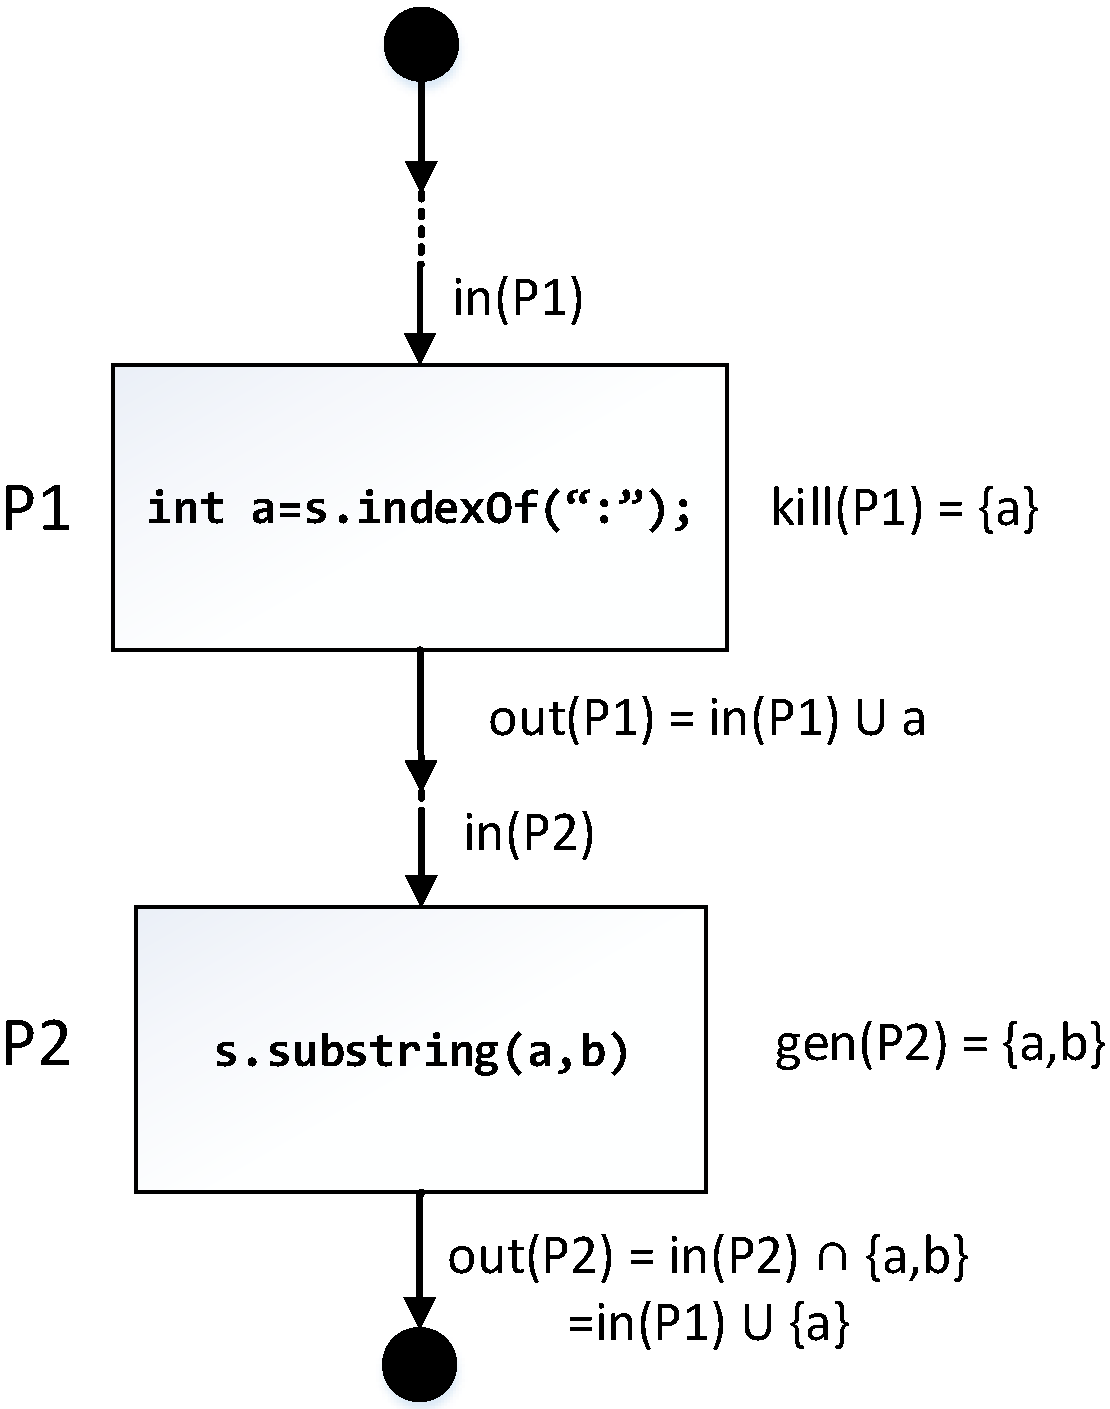
\includegraphics[scale=.30]{images/dataflow.png}
\caption{Dataflow diagram with in, out set in forward analysis}
\label{fig:dataflow}
\end{figure}

\subsubsection{Flow Function}
\label{subsubsec:flowFunction}

~\newline
Let us define $P_i$ as a program point/ node in the control flow graph. $in(P)$
and $out(P_i)$ respectively denotes in set and out set to and from the node $P$.
We define set $IG$ as the set of methods like \code{indexOf()},
\code{codePointAt()}, \code{CodePointBefore()} etc. which returns an integer
which can be used as input to other String methods. We also define set $IU$
which contains the methods which may use the integers produced by the methods in
$IG$ Then, 
$$out(P_i) = in(P_i) \cup Def(P_i)$$ where statement in P is a invoke statement
and method $m \in IG$ and
$$out(P_i) = in(P_i) \cap Used(P_i)$$ where statement in P is a invoke statement
and method $m \in IU$. Initial entry set = ${\phi}$.


We have defined $Def(P_i)$ set as the set of variables and objects which are
defined or redefined in the program point $P_i$. The set $Used(P_i)$ is also a
set of variables and objects which are used in the program point $P_i$.

\textbf{Example}: Consider the program statement \code{Pi : int a = b.fun(c
d)}.
Here the variable \code{a} is initialized, so $Def(P_i)$ = \code{\{a\}} and
as
\code{b, c, d} are used, $Used(P_i) =$ \code{\{b, c, d\}}

In the figure~\ref{fig:dataflow}, we gave an example of a sample CFG with in set
and out set.
}

\subsubsection{Constraint Storage}
\label{subsubsec:constraintStorage}

~\newline
For each of the string object, we store in the way illustrated in the
Figure~\ref{fig:constraint}.

\begin{figure}[t]
\centering
%% change the font size in the img; make it min len, max len
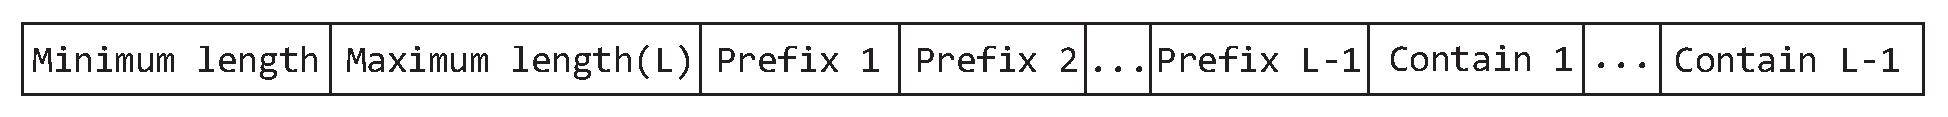
\includegraphics[width=\linewidth]{images/constraint.eps}
\caption{String constraints storage format}
\label{fig:constraint}
\end{figure}

When to evaluate a new string object we need bounds like the minimuma and maximum
length, the prefixes and the candidate characters and their relative position.
We keep minimum information to safely evaluate the string.

\begin{algorithm}
\scriptsize
\DontPrintSemicolon
\KwData{String object $Str$ and constraint set $CS$.}
\KwResult{String object $Str$ such that $\forall i \in CS$, $Str$ satisfies $i$
}
\Begin
{
 $CS_{Str} \longleftarrow$ Get the constrint set for $Str$\;
 $MinLength \longleftarrow CS_{Str}[0]$\;
 $MaxLength \longleftarrow CS_{Str}[1]$\;
 $PrefixSet_{Str} \longleftarrow CS_{Str}[2 \rightarrow MaxLength + 1]$\;
 $ContainSet_{Str} \longleftarrow CS_{Str}[MaxLength +2  \rightarrow 2*MaxLength
 + 1]$\;
 
  \For{$C \in PrefixSet_{Str}$}
  {
   \If{$C$ is Empty}
   {
    continue\;
   }
   $PrefixLength \longleftarrow$ {\bf LENGTH OF} $C$\;
   
   \If{$PrefixLength$ is Maximum $\in PrefixSet_{Str}$}
   {
     Use $C$ to construct $Str$\;
   }
  }
 
  \For{$C \in ContainSet_{Str}$}
  {
   \If{$C$ is Empty {\bf OR} $C \in Str$}
   {
    continue\;
   }
   $Str \leftarrow Str$ {\bf APPEND} $C$\;
  }
  return $Str$\;
}
\caption{String object constraint evaluation}
 \label{algo:constraint}
\end{algorithm}

\subsubsection{Repairing Strategy using Constraint Evaluation}
\label{subsubsec:repairingStrategyConstraint}

~\newline
The patching is evaluated in two ways, static and dynamic. We evaluated those
conditions which can be evaluated safely during compile time. Such constraints
have constants like \code{if(s.length<10)}. We looked for particular
constraints based on our storage specification. In the algorith~\ref{algo:constraint}
we describe one such evaluation technique with \code{String} objects.

\begin{algorithm}
\scriptsize
\DontPrintSemicolon
\KwData{Set of conditional statement on string $str$}
\KwResult{Constraint set $CS_{str}$}
\Begin
{ 
  \For{Conditional statement$ \leftarrow i$, $\forall i \in CS_{str}$}
  {
   $i \Rightarrow str\ *\ OP$\;
   where $*$ is the binary comparisn operator\;
   \If{$*$ is $==$}
   {
    $maxlength_{str} \longleftarrow OP$\;
    $minlength_{str} \longleftarrow OP$\;
   }
   
   \If{$*$ is $\textgreater$ {\bf AND} $*$ is $\ge$}
   {
    $minlength_{str} \longleftarrow OP$\;
   }
   
   \If{$*$ is $\textless$ {\bf AND} $*$ is $\le$}
   {
    $maxlength_{str} \longleftarrow OP$\;
   }
   
   \If{$*$ is Prefix Check}
   {
    $PrefixSet_{str} \cup OP$\;
   }
   
   \If{$*$ is Contains Check}
   {
    $ContainSet_{str} \cup OP$;
   }
  }
}
\caption{Constraint collection for \code{String} objects}
 \label{algo:constraintCollection}
\end{algorithm}

\begin{algorithm}
\scriptsize
\DontPrintSemicolon
\KwData{Control flow graph $CFG$ for program $P$}
\KwResult{Patched program $\hat{P}$}
\Begin
{ 
 \For{$\forall$ node $N \in CFG$}
 {
  Statement $S$ in node $N$\;
  \If{$S$ conntaints \code{String} API call}
  {
  	$str \longleftarrow$ \code{String} reference on $S$\; 
  	\If{$S$ can throw \code{RuntimeException}}
  	{
  		Exception class $EC \longleftarrow$ \code{RuntimeException} of $S$\;
  		$CES_{str} \longleftarrow$ all conditional statement in $P$ on $str$;
  		$CS_{str} \longleftarrow$ output of
  		Algorithm~\ref{algo:constraintCollection}$(CES_{str})$ \;
  		\If{$str$ have sufficient constraints in $CS_{str}$}
  		{ 
  			$str \longleftarrow$ output of Algorith~\ref{algo:constraint}$(CS_{str})$\;
  		}
  		\Else
  		{
  			$str \longleftarrow$ output of
  			Algorithm~\ref{algo:stringPatchParametr}$(S)$\; 
  		}
  		Instrument ~\ref{algo:constraintCollection}$(CES_{str})$ in $P$ for dynamic
  		constraint collection\;
  		Instrument ~\ref{algo:constraint}$(CS_{str})$ in $P$ for dynamic
  		constraint evaluation\;
  	}
  } 
 }
}
\caption{Patching strategy for \code{String} objects}
 \label{algo:patchingStrategy}
\end{algorithm}